\documentclass[11pt,a4paper]{article}
\usepackage{fullpage}
\usepackage{graphicx}
\usepackage{siunitx}
\usepackage{amsmath}
\usepackage{bm}
\usepackage[hidelinks]{hyperref}
\usepackage[noabbrev, capitalise]{cleveref}

\title{Consideration of objects between a camera and the target for infrared measurements}

\author{Andrew Hurlbatt}

\date{\today}

\renewcommand{\abstractname}{\vspace{-\baselineskip}}

\begin{document}
	
	\maketitle
	
	\begin{abstract}
		In making infrared measurements, it is usually the case that objects, including air, exist between the camera and the target that affect the infrared radiation between the two. In addition, all objects reflect some amount of radiation from the environment. A method is detailed here of using summary properties of the objects involved to estimate the actual radiance emitted by the target. Self-emission, transmittances, and reflectances of all objects are considered, also allowing for reflections between objects.
	\end{abstract}

When using infrared imaging to measure object temperatures, there are often objects along the imaging path that may alter the radiation through absorption, reflection, or addition of their own emission. These should all be taken into account when using a measured radiance to estimate that of a target. In this work, the properties of each object are assumed to be single values, and should therefore be calculated with the spectral response of the detector included. 

An example system is shown in \cref{fig:scheme}, indicating that each object $ n $ out of $ N $ objects can have its own radiance $ M_n $, emittance $ \epsilon_n $, transmittance $ \tau_n $, specular reflectance $ \rho_n $, and diffuse reflectance $ \sigma_n $. Object radiances are generally taken to be that of a black body at the same temperature, as wavelength dependant emittances are seldom known. Also defined are the properties of the target (with subscript $ T $), radiance of the background around the system $ M_B $, the emission measured by the camera $ M_M $, and $ F_n $ and $ B_n $, being the forward and backward travelling radiation, respectively, between objects $ n $ and $ n+1 $.

\begin{figure}
	\centering
	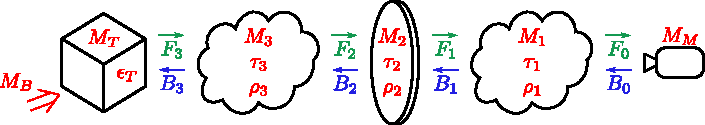
\includegraphics[width=\textwidth]{./infroptics_scheme.pdf}
	\caption{An example system with a window between the camera and the target, showing the atmosphere between each object should also be considered.}
	\label{fig:scheme}
\end{figure}

From this arrangement, one can begin to define the quantities $ F_n $ and $ B_n $ in a recursive manner based on the properties of the objects. The quantity $ F_{n-1} $ must be the result of the interaction of object $ n $ with $ B_{n-1} $ and $ F_{n} $, leading to \cref{eq:Fn-1,eq:Fn}.

\begin{align}
	F_{n-1} &= \rho_n B_{n-1} + \tau_n F_n + \epsilon_n M_n + \sigma_n M_B \label{eq:Fn-1} \\
	F_n &= \frac{F_{n-1} - \rho_n B_{n-1} - \epsilon_n M_n - \sigma_n M_B}{\tau_n}\label{eq:Fn}
\end{align}

Similarly, $ B_n $ also results from the same interaction, but in the other direction, as given in \cref{eq:Bn}.

\begin{equation}\label{eq:Bn}
	\begin{split}
		B_n &= \rho_n F_n + \tau_n B_{n-1} + \epsilon_n M_n + \sigma_n M_B \\
		&= \rho_n \frac{F_{n-1} - \rho_n B_{n-1} - \epsilon_n M_n - \sigma_n M_B}{\tau_n} + \tau_n B_{n-1} + \epsilon_n M_n + \sigma_n M_B \\
		&= \frac{\rho_n}{\tau_n} F_{n-1} + \left(\tau_n - \frac{\rho_n^2}{\tau_n}\right) B_{n-1} + \left(1 - \frac{\rho_n}{\tau_n}\right) \left(\epsilon_n M_n + \sigma_n M_B\right)
	\end{split}
\end{equation}

The pair of coupled recursive equations \cref{eq:Fn,eq:Bn} are linear in $ F_{n-1} $ and $ B_{n-1} $, and can be turned into a single recursive matrix equation, \cref{eq:mat}, by defining the matrices that follow.

\begin{align*}
	\bm{X}_n &=
	\begin{bmatrix}
		F_n \\ B_n
	\end{bmatrix}
	&
	\bm{A}_n &=
	\begin{bmatrix}
		\frac{1}{\tau_n} & -\frac{\rho_n}{\tau_n} \\
		\frac{\rho_n}{\tau_n} & \tau_n-\frac{\rho_n^2}{\tau_n} \\
	\end{bmatrix}
	&
	\bm{b}_n &= 
	\begin{bmatrix}
		-\frac{\epsilon_n M_n + \sigma_n M_B}{\tau_n}\\[4pt]
		\left(1 - \frac{\rho_n}{\tau_n}\right) \left(\epsilon_n M_n + \sigma_n M_B\right)
	\end{bmatrix}
\end{align*}

\begin{equation}\label{eq:mat}
	\bm{X}_{n} = \bm{A}_n \bm{X}_{n-1} + \bm{b}_n
\end{equation}

With the relatively light assumption that $ F_0 = M_M $ and that $ B_0 = 0 $ (i.e. negligible radiation is travelling from the camera back toward the target), $ \bm{X}_0 = \left[ M_M \enspace 0\right]^T$, and the system can be solved iteratively if the properties of all objects (apart from the target) are known.

To avoid iterative solutions, the recursion can be unravelled into a single formula, given in \cref{eq:full_matrix}. In this and following expressions, ``Big-Pi'' notation is used to mean matrix multiplication, with subsequent terms being ordered left to right.

\begin{equation}\label{eq:full_matrix}
	\bm{X}_n = \left(\prod_{i=1}^n \bm{A}_{n-i}\right) \bm{X}_0 + \sum_{i=0}^{n-2} \left( \prod_{j=1}^{n-i-1} \bm{A}_{n-j} \right) \bm{b}_i + \bm{b}_n
\end{equation}

By isolating the two constant terms, they can be taken out of the expression and evaluated individually to give a single, non-recursive, expression for $ \bm{X}_N $ in \cref{eq:X_N}, from which the value of $ F_N $ can be extracted.

\begin{align*}
	\bm{D}_n &= \prod_{i=1}^n \bm{A}_{n-i} &
	\bm{C}_n &= \sum_{i=0}^{n-2} \left( \prod_{j=1}^{n-i-1} \bm{A}_{n-j} \right) \bm{b}_i + \bm{b}_n
\end{align*}

\begin{equation}\label{eq:X_N}
\bm{X}_{N} = \bm{D}_N \bm{X}_0 + \bm{C}_N
\end{equation}

The value of $ F_N $ does not immediately give us the estimated object radiance however, as it is also reflecting some radiance from the background and from $ B_N $. The quantity $ M_T $ is the radiance after correcting for this, and is given in \cref{eq:M_T}.

\begin{align}
	M_T &= \frac{F_N - \sigma_T M_B - \rho_T B_N}{\epsilon_T} \nonumber\\
	M_T &= \frac{1}{\epsilon_T} F_N - \frac{\rho_T}{\epsilon_T} B_N - \frac{\sigma_T}{\epsilon_T} M_B \nonumber\\
	M_T &= \begin{bmatrix} \frac{1}{\epsilon_T} & - \frac{\rho_T}{\epsilon_T} \end{bmatrix} \bm{X}_{N} - \frac{\sigma_T}{\epsilon_T} M_B \label{eq:M_T}
\end{align}

\begin{align*}
\bm{P}_T &= \begin{bmatrix} \frac{1}{\epsilon_T} & - \frac{\rho_T}{\epsilon_T} \end{bmatrix} &
\bm{K} &= \bm{P}_T \bm{D}_N &
l &= \bm{P}_T \bm{C}_N - \frac{\sigma_T}{\epsilon_T} M_B
\end{align*}

\begin{equation}\label{eq:K}
	M_T = \bm{K} \bm{X}_0 + l
\end{equation}

By collecting terms into \cref{eq:K}, and extracting $ M_M $ as the first element of $ \bm{X}_0 $, one arrives at a linear relationship between the measured radiance $ M_M $ and the estimated radiance of the target object $ M_T $, with coefficients that are fully determined by the properties of the $ N $ objects and the radiance of the background. This is given in \cref{eq:M_T_M_M}, where $ k_{1} $ is the first element of $ \bm{K} $.

\begin{equation}\label{eq:M_T_M_M}
	M_T = k_{1} M_M + l
\end{equation}

The coefficients of the linear expression in \cref{eq:M_T_M_M} are independent of the measured radiance, and therefore only need to be calculated once for each system, which can improve efficiency.

\end{document}